\documentclass[12pt] {article}
\usepackage{hyperref}
\usepackage{graphicx}
\newtheorem{definition}{Definition}

\begin{document}

%Title page
\begin{titlepage}
    \centering
    \vspace{.7\baselineskip}
    {\huge \textbf{Morally correct way of solving SAT}}
\end{titlepage}

\newpage

%Abstract
\section{Abstract}
% Motivation could be said here
SAT is a decision problem where we need to determine whether is a given Boolean formula in conjunctive normal form (CNF) is satisfiable. The problem is NP-complete, which means that there isn’t a known algorithm which could efficiently solves SAT problem.

% The MiniSAT, ManySAT parts can be freely changed, there is no such thing as sharing graph. Also combining them might not even make sense.
The Sequential SAT based on the David-Putnam-Loveland-Logemann (DPLL) algorithm. Later the improvements in CDCL(Conflict Driven CLause Learning) and "restart" technique led to the MiniSAT. The MiniSAT provided schema for Parallel SAT-Solvers. The ManySAT is a parallel SAT-Solver and it made the portfolio SAT Solvers popular. ManySAT's weakness is the problem with sharing between slaves. Our method improves on previous methods by MiniSAT and ManySAT, by solving the issues of sharing. ManySAT works by running many SAT instances on a partitioned searchspace. MiniSAT works in a grid model, but has no sharing. We combine the sharing and grid based methods. We archive this by sharing graphs that share information on conflicting clauses.

% End of the abstract, results in advance
The testing results of the algorithm demonstrate its efficiency and accuracy on various benchmark SAT problems. The new approach significantly reduced the runtime compared to classical methods. The potential of the algorithm is further proven by its ability to handle more complex instances.

\section{Introduction}
% SAT summarized
The Boolean Satisfiability Problem  is one of the most important and fundamental problem in Computer Science. Especially in the theory of algorithms and computational complexity. The point of the problem to decide, whether does exist a variable combination (True, False values), that satisfies a given logical formula, that contains more than one different variable and more than one binary logical operator. The problem is the first instance of the NP-complete category and plays a key role in NP problems examination.

% History of SAT
The history of SAT started in the 19. century. Boole algebra and logic domains founded, which made it possible to express logical operations in algebraic form. This evolved the modern computer logic and the basics of SAT problem. In the early 1900s, the works of Alan Turing and Kurt Gödel helped the formalization of problems like SAT and the analysis of the algorithms. In 1971 Stephen Cook published, that the SAT is and NP-complete problem, which means non-deterministic polynomial time problem. It follows, that every NP-problem traceable to SAT in polynomial time. This was the first time in history, when SAT was considered as a NP-complete problem. From the 1980s to the present day, due to the practical applications the demand of SAT solver efficient algorithms has increased. From the late 80s and 90s the evolution of the SAT solvers was extremely fast. On the one hand DPLL algorithm and it's different modifications, and on the other hand the conflict based learning techniques brought a breakthrough.
% Important progresses and methods SAT solvers
\\Some of the most important advances and methods in SAT solvers:
\begin{itemize}
    \item In 1962 the DPLL (Davis-Putnam-Logemann-Loveland) algorithm was published. It was the first efficient SAT solver, that searches for solutions systematically to the logical formula with tracing back and ramification.
    \item The modern SAT solvers often use heuristic methods to reduce the seeking space, to find satisfying solutions quickly. For instance the VSIDS (Variable State Independent Decaying Sum) is an often used decision heuristic.
    \item Conflict-Driven Clause Learning, CDCL is one of the most important innovator, that made possible to solve more complex problems. The algorithm tries to learn from conflicts, that occur during execution to avoid unnecessary searches.
    \item In the late 90s, the Stochastic Local Search algorithm tries to solve the problem with heuristic approach. And works efficiently in the practical SAT cases.
\end{itemize}
% SAT praktical usage
The SAT problem solution has many fields of application, such as:
\begin{itemize}
    \item \textbf{Hardware and software verification:} The logical electric circuits and the programs formal control.
    \item \textbf{Code optimization and automated planning:} Solutions often used in optimization tasks such as automated planning.
    \item \textbf{Cryptography:} SAT solver algorithms play key roles in cryptography algorithms security analysis.
\end{itemize}


%Related works
\section{Related works}

\subsection{Stochastic Boolean Satisfiability}

The article of Stochastic Boolean Satisfiability presents a connection point between a satisfiability problem and a probabilistic model. It Demonstrates how to adapt a view of satisfiability on the field of probability. SSAT in focus, a general stochastic satisfiability problem, which plays a similar role in probabilistic domains like SAT in deterministic ones.The article analyze the relationship between planning and uncertainty. Shows systematic and stochastic algorithms, for SSAT solutions. Perhaps the complexity gap between SSAT (PSPACE) and SAT (NP), is large, the article suggests, that the knowledge of SAT could be applied to the probabilistic domain.

\subsection{A survey of SAT solver}

In Computer Science, the Boolean Satisfiability Problem(SAT) is the problem of determining if there exists an interpretation that satisfies a given Boolean formula. SAT is one of the first problems that was proven to be NP-complete, which is also fundamental to artificial intelligence, algorithm and hardware design. This paper reviews the main algorithms of the SAT solver in recent years, including serial SAT algorithms, parallel SAT algorithms, SAT algorithms based on GPU, and SAT algorithms based on FPGA. The development of SAT is analyzed comprehensively in this paper. Finally, several possible directions for the development of the SAT problem are proposed.

\subsection{Sequential SAT Solvers}

The first SAT Solvers were sequential ones. These based on the Davis-Putnam-Loveland-Logemann (DPLL) algorithm. This algorithm includes rules which help to generate and traverse a binary search tree. Each part of the search tree is equal to a partial interpretation. The tree's branch elements walked through by a back-track algorithm and the main goal is to explore recent alternatives. This led to the CDCL (Conflict Driven Clause Learning) algorithm. The algorithm resolve the conflict clause and those clauses which were used in the implications, and learn these ones. After, these clauses can be added to the further formulas and improve the backtracking behaviour. Another technique was the "restarts", which helped to upgrade the performance. The most common SAT Solver which combine the CDCL and restart technique is the MINI-SAT. The MINI-SAT was introduced in 2003 and got improvements in each year and provided a basic schema, for sequential and parallel SAT-Solvers.


\subsection{An overview of parallel SAT solving}

In recent years the multicore architectures are becoming more and more wide\-spread. The SAT solvers should take advantage of this. Therefore, researchers have put a lot of focus on parallel algorithms. In the An overview of parallel SAT solving article we can read a great summary of the results in this field. The paper demonstrates the search space splitting and portfolio strategies which are the most important approaches. Furthermore, it contains some other significant solutions, for example hybrid methods. The different techniques present how multicore architectures can be used in SAT solving, and these had a relevant impact on our research.


\subsection{Parallel SAT Solvers}

At the dawn of the Parallel SAT Solvers, the first Solver only used single-core CPU, and communicated via network. When the memory sharing architectures became available, the scientists made studies on which is faster and supplemented the Parallel SAT Solver with more CPU cores and memory. The first impressions were really great, but later they found out, that if you use too many CPU cores and memory sharing, the efficiency decreases, because of the latency with the shared memory parts and the search for the optimal core slows down the software. The root of the problem was that the solver couldn't handle the underlying hardware very well and the calculations on the other cores wasn't perfectly balanced. So this helped to identify the principles what a many-core SAT Solver should achieve, in order to be an efficient Parallel SAT Solver:
1. The solver should aware of the hardware components in order to utilize the non-uniform access.
2. The solver should exchange the learned clauses and the data between the processes which running on different cores and has to be balanced well from the calculus up to the hardware level.
So lastly, if you want to create a well designed parallel SAT Solver, you must have a redesigned and reviewed Sequential Solver. It is still an open question that how you can build an efficient SAT Solver with a high level of scalability, combined with the modern multi-core architecture.
Our work is far from that to be honest, but we made the first step towards a more efficient and more scaleable parallel SAT Solver. The next topic will explain how and what we did to make the humanity closer to this desire.

%Background
\section{Background}
SAT problem is about satisfiability of Boolean formulas in conjunctive normal form (CNF). The necessary definitions for this can be read below. The definitions are valid in propositional logic.
\subsection{Boolean formulas and satisfiability}
\begin{definition}
In propositional logic we use symbols to represent propositions, these symbols called propositional variable which can be true or false.
\end{definition}
\begin{definition}
Interpretation is a function which maps propositional variables to logical values (true or false). In other words, the interpretation determines whether the value of a variable is true or false).
\end{definition}
\begin{definition}
\begin{enumerate}
    \item Every propositional variable is a formula.
    \item If $X$ is a formula, then $\neg X$ is a formula too, where $\neg $ is the sign of negation.
    \item If $X$ and $Y$ is a formula, then $(X \circ Y$) is a formula too, where $\circ$ can be $\wedge$ (conjunction) or $\vee$ (disjunction) or $\supset$ (implication).
\end{enumerate}
Every formula is created by using the previous rules finitely many times.
\end{definition}
\begin{definition}
An interpretation satisfies a formula if the formula is true in that interpretation.
\end{definition}
\begin{definition}
A formula is satisfiable, if exists an interpretation which satisfies it, otherwise it is unsatisfiable.
\end{definition}
\subsection{Conjunctive normal form}
\begin{definition}
A propositional variable ($X$) and its negated form ($\neg X$) are called literals.
\end{definition}
\begin{definition}
A disjunction of literals is called clause.
\end{definition}
\begin{definition}
A conjunction of literals is a formula is in conjunctive normal form (CNF).
\end{definition}


%test results and analysis
\section{Measurements}
In this section below, the test results of the new algorithm can be seen. The SAT problem is NP-complete, which means most of the modern algorithms' computational cost are close to exponential. But our method provides $n^{2}$ computational cost.

\subsection{Test results}
During testing we ran our algorithm and one of our most efficient on SAT problems. We tried the algorithms on logical formulas, that contains 1 to 4 logical variables. The methods got the same formulas, problems. The results of the executions are shown the diagrams below.

On the diagrams the blue dots represents our algorithm max and min computational costs for each amounts of logical variables. The red dots represents the concurrent algorithms minimal computational cost. The blue line shows the average costs of our algorithm, the read one belongs to the best concurrent algorithms. For instance the SAT-3 problem solved in only 9 steps.

\begin{figure}[h]
    \centering
    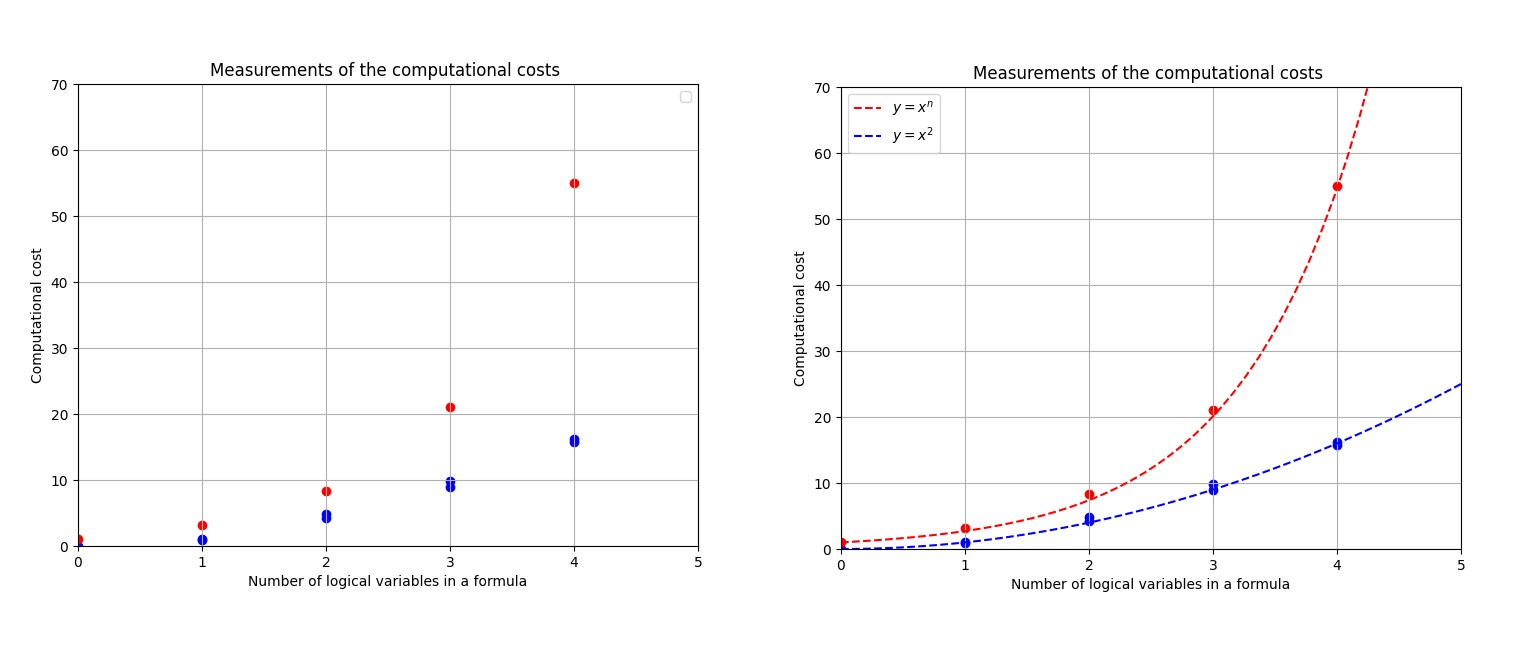
\includegraphics[width=1\linewidth]{img/measurements.png}
\end{figure}

\subsection{Analysis}
It seems, that due to the dissimilar average computational costs, major magnitude differences formed. The new method for SAT solution, provides $n^{2}$ computational cost, because of the advanced heuristic model.This cause a great advantage against the concurrent algorithms.

%future work
\section{Future work}

We earned great results with our methodology, but the algorithm still can be faster.
In future we would like to optimize further the computational costs and the runtime.
We will continue our research in this direction.

\newpage
\section{Bibliography}

[1] - \href{https://link.springer.com/article/10.1023/A:1017584715408}{Stochastic Boolean Satisfiability}
\newline
[2] - \href{https://doi.org/10.1063/1.4981999}{A survey of SAT solver}
\newline
[3] - \href{https://link.springer.com/article/10.1007/s10601-012-9121-3}{An overview of parallel SAT solving}
\newline
[4] - \href{https://www.researchgate.net/publication/254048189_A_short_overview_on_modern_parallel_SAT-solvers}{A short overview on modern parallel SAT Solvers}

\end{document}
    